\section{Case study}
\label{sec:case_study}
\subsection*{Patterns of multi-controller failure cases}

\paragraph*{How are these failures created at the first place?}
Large systems are developed by people in different teams and different organizations. One team or a certain group of people in case of open source is responsble for developing and maintaining a certain part out of the entire system. It is impossible for them to know how all other parts of the system function in detail. It is not feasible to write a controller not incuring any conflicted cases with all other controller for all possible cases. Even if it is technically possible, it is not even desirable because then the development process will take exhastively long time.
The programming model of the large system including Kubernetes is another contributer to this type of failure. We will use Kubernetes to describe more detailed example. What each controller does in Kubernetes is periodically monitoring if the associated part in the cluster is currently in desirable status or not. If it is not, it will try to bring it back to the desirable status, running built-in logic of the controller. For example, Horizontal Pod Autoscaler(HPA) scales up the number of pods if CPU utilization becomes higher than 50\% (it is configurable). This specific model is called reconciliation. During reconciliation The important part is a controller does not take into account what other controllers are doing and how they can react to its action. It simply sees the current status of the cluster and run its own logic to put the cluster back to the right place.
Even within one controller, there could be multiple configurations which are functionally not exclusive each other. For exapmle, Deployment could be configured with multiple \textit{Pod Topology Spread Constraint} policies and currently Kubernetes does not have safety net guaranteeing that the configurations are not contradictorial or any kind of alerting system warning it is contradictorial. It is completely at your own risk.


\paragraph*{Why is it hard to prevent these failures?}
If it is evident that the system could fall into already known precarious status when the cluster is deployed with self-destroying configuration, why were they not fixed already? It is not because it is such a huge system and the community is large enough or active to resolve these problems. It is because they are not trivial problems. Note that each part of the system is not doing anything wrong if you look at them individually and there is no bug in the code.
It is inherently ambiguous to classify such failure cases as bug. Each controller is working as it is supposed to do and clearly there is no bug in its logic if you look them individually. Some of answers against reported github issues was that developers in Kubernetes community maintaining the controller are aware of or admit that is the issue but they ended up not fixing or not being able to fix it while saying it is their design choice or there is no clear way to patch it. The clear solution does not exist since multiple parties in the system are involved and tangled each other. It is not because Kubernetes community constantly procrastinates or neglects them. 
Most of these problems we are presenting in this paper could be prevented if you know it will happen before you apply them to your cluster. For the example in D1 failure case, if you had known that Deployment configuration and Scheduler policy are contradictorial each other, you would have not configured in such self-destroying way. However, there are several reasons that it is still not trivial to avoid this type of failures. The first reason is scalability. The nubmer of pods could be easily over a thousand and the number of services deployed in the cluster could be easily over a hundred. To configure this scale of Kubernetes cluster having different applications running, you may need to manage a large number of configuration yaml files for each deployment, nodes, hpa, schedulers, etc. In this scale and complexity, it is challenging to make all controllers always in a coordinated manner in the cluster-wise level. The second reason is that in a large scale cluster some failrues are not noticeable and slowly gnawing the cluster's resources. For example, in S1 failure case, node utilization on average could stay within some range in the half way of scheduler config and deschduler config. It is possible that the cluster resource utilization looks stable even though what is happening beind is deschduler keeping evicting pods from high utilization node and scheduler placing pods in low utilization node makig the utilization high again. The third reasons is that semantically contradictorial configurations does not mean it will always lead to failrues. Many of these problems are triggered in a specific number of nodes and pods. 

\begin{table*}[t]
    \centering
    \begin{tabular}{c c c c c c}
    \hline
        Case & Categories & Controllers & Properties & Behaviors  \\ 
        \hline
        D1(R) & Conflicted config & Deployment + Kubelet & Liveness & Scheduling and evicting pods infinitely  \\ 
        H1(R) & Lack of context & HPA + App CPU changes & Safety & HPA is agnostic to app  \\ 
        H2(R) & Conflicted config & HPA + Deployment & Safety & Sub-optimal scaling behavior  \\ 
        H3(R) & Imperfect knowledge & HPA + Node reachability & Safety & Semantically wrong avg CPU util (reachability vs healthiness)  \\ 
        S1 & Conflicted config & Scheduler + Descheduler & Liveness & High utilization(scheduler) <-> Low utilization(descheduler) \\ 
        S2(R) & Conflicted config & Scheduler + Descheduler & Liveness & Deployment preference <-> Violation in maxSkew \\ 
        S3(R) & Conflicted config & Scheduler & Liveness & Two pod spread constraints are conflicted each other  \\ 
        S5 & Conflicted config & Scheduler & Safety & Pods are scheduled to one node, because of lopsided preference  \\ 
        S6(R) & Lack of feature & Scheduler & Safety & Scheduler is not able to adjust skewed placement  \\ 
        S7(R) & Lack of context & Scheduler + Kubelet & Liveness & Scheduler includes NotReady node for maxSkew calculation  \\ 
        \hline
    \end{tabular}
    \caption{}
    \label{table:summary}
\end{table*}

\subsection*{Detailed examples}

\begin{figure}[h]
    \centering
    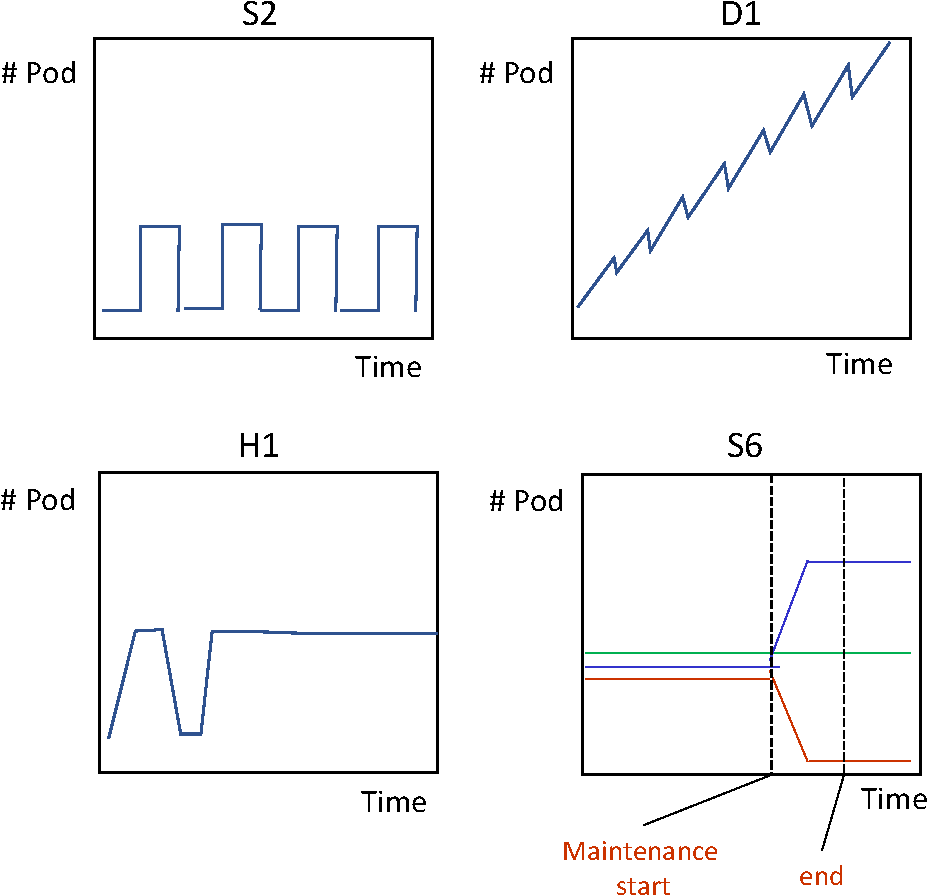
\includegraphics[width=0.4\textwidth]{figure/num_pod.pdf}
    \caption{Number of pods over time for four failure cases.}
    \label{fig:num_pod}
\end{figure}


\subsection*{Observation 1}
